% Тип документа
\documentclass[a4paper,14pt]{extarticle}

% Шрифты, кодировки, символьные таблицы, переносы
\usepackage[utf8]{inputenc}
\usepackage[russian]{babel}
% Это пакет -- хитрый пакет, он нужен но не нужен
\usepackage[mode=buildnew]{standalone}

\usepackage
    {
        % Дополнения Американского математического общества (AMS)
        amssymb,
        amsfonts,
        amsmath,
        amsthm,
        % Пакет для физических текстов
        physics,
        % misccorr,
        % 
        % Графики и рисунки
        wrapfig,
        graphicx,
        subcaption,
        float,
        caption,
        color,
        booktabs,
        geometry,
        % 
        % Таблицы, списки
        makecell,
        multirow,
        indentfirst,
        %
        % Интегралы и прочие обозначения
        ulem,
        esint,
        esdiff,
        % 
        % Колонтитулы
        fancyhdr,
    } 
    
\usepackage{mathtools}
\mathtoolsset{showonlyrefs=true} 

\usepackage{xcolor}
\usepackage{hyperref}
\usepackage{pythontex}
 % Цвета для гиперссылок
\definecolor{linkcolor}{HTML}{000000} % цвет ссылок
\definecolor{urlcolor}{HTML}{799B03} % цвет гиперссылок
 
\hypersetup{linkcolor=linkcolor,urlcolor=urlcolor, colorlinks=true}
\hypersetup{pageanchor=false}
% Увеличенный межстрочный интервал, французские пробелы
\linespread{1.3} 
\frenchspacing 

\newcommand{\mean}[1]{\langle#1\rangle}
\newcommand\ct[1]{\text{\rmfamily\upshape #1}}
\newcommand*{\const}{\ct{const}}
\newcommand{\tK}{\widetilde K}

\usepackage{array}
\usepackage{pstool}

\geometry       
    {
        left            =   2cm,
        right           =   2cm,
        top             =   2.5cm,
        bottom          =   2.5cm,
        bindingoffset   =   0cm
    }

%%%%%%%%%%%%%%%%%%%%%%%%%%%%%%%%%%%%%%%%%%%%%%%%%%%%%%%%%%%%%%%%%%%%%%%%%%%%%%%
    %применим колонтитул к стилю страницы
\pagestyle{fancy} 
    %очистим "шапку" страницы
% \fancyhead{} 
    %слева сверху на четных и справа на нечетных
\fancyhead[R]{\small Понур К.А.}%\labauthors 
    %справа сверху на четных и слева на нечетных
% \fancyhead[L]{Отчёт по лабораторной работе №\labnumber}
\fancyhead[L]{Кафедра общей физики} 
    %очистим "подвал" страницы
% \fancyfoot{} 
    % номер страницы в нижнем колинтуле в центре
\fancyfoot[C]{} 

%%%%%%%%%%%%%%%%%%%%%%%%%%%%%%%%%%%%%%%%%%%%%%%%%%%%%%%%%%%%%%%%%%%%%%%%%%%%%%%

\renewcommand{\contentsname}{Оглавление}
\usepackage{tocloft}
\usepackage{secdot}
\sectiondot{subsection}


\begin{document}
\section{Общие понятия}%
\label{sec:obshchie_poniatiia}

Рассмотрим ряд общих понятий, описывающих возвышения взволнован-
ной морской поверхности в рамках теории случайных пространственно-временных
полей. Представим возвышения поверхности в виде суммы гармонических бе-
гущих волн с независимыми фазами:
\begin{equation}
    \label{eq:surface}
    \xi(\vec r,t) = \sum\limits_{n=-\infty}^{\infty} 
    A_n(\vec k_n) \exp{i(\vec k_n \vec r)},
\end{equation}
где $A_n (\vec k_n)$ -- комплексная амплитуда гармоники с волновым числом
$\vec k_n$ и временной частотой  $\omega_n$, связанной с  $\vec k_n$ известным
дисперсионным соотношением  $\omega = \omega(k)$.

Корреляционную функцию поля  $\xi(\vec r, t) $ определим как
 \begin{equation}
    \label{eq:corr}
    K_{\xi}\qty[\vec r_1, \vec r_2, t_1,t_2] = \mean{\xi(\vec r_1,t_1)\xi^*(\vec r_2,t_2)}
\end{equation}

Поле высот в нашей задаче считаем стационарным в широком смысле, то есть 
$K_{\xi}\qty[\vec r_{1},\vec r_{2},t_{1},t_{2}] = K_{\xi}\qty[\vec \rho = \vec
r_{2} - \vec r_1, \tau=t_{2}-t_{1}]$. Корреляционную функцию поверхности
\eqref{eq:surface} несложно посчитать
\begin{equation}
    \label{eq:surface_corr}
    K_{\xi}\qty[\vec \rho,\tau] = \sum\limits_{n=-\infty}^{\infty} 
    \frac{(A_n (\vec k_n))^2}{2} \exp{i \qty(\vec k_n \vec \rho - \omega \tau)}
\end{equation}

В дальнейшем мы будем рассматривать мгновенный снимок моделируемой поверхности,
а значит положить $\tau = \const = 0$  и  $K_\xi[\rho,\tau] = K_\xi [\rho]$.

Тогда справедлива формула Винера-Хинчина
\begin{equation}
    \label{eq:Viner-Hinchin}
    S_\xi(\vec k) \int\limits_{-\infty}^{\infty} K_\xi \qty[\vec \rho] e^{- i
    \vec k \vec \rho} \dd \rho. 
\end{equation}

Будем полагать, что волновой спектр имеет вид функции с разделяющимися
переменными
\begin{equation}
    S_\xi(\vec k) = S_\xi(k) \Phi(\phi),
\end{equation}
где $k = \sqrt{k_x^2 + k_y^2}$,  $\phi = \arctg \frac{k_x}{k_y}$. Для удобства,
нормируем угловое распределение $\int\limits_{-\infty}^{\infty} \Phi(\phi) \dd
\phi = 1$.

Спектр мощности $S_\xi(k)$ и азимутальное распределение  $\Phi(\phi)$ известны
из экспериментов (см. [пример 1]). Практическую реальзацию построения модели
морсксой поверхности мы рассмотрим далее.

\section{Двумерная модель поверхностного волнения}%
\label{sec:dvumernaia_model_poverkhnostnogo_volneniia}

В соответствии с предыдущим разделом, для моделирования случайной повехрности
$\xi(\vec r,t)$ будем исполььзовать её представление в виде суперпозиции
плоских волн с различными частотами и случайными фазами $\psi_{nm}$, бегущих
под разными азимутальными углами $\phi_m$ \cite{kekke}:
\begin{equation}
    \label{eq:surface2d}
    \xi(\vec r,t) = \sum\limits_{n=1}^{N} \sum\limits_{m=1}^{M} A_n(k_n) \cdot
    F_m(\phi_m) \cos \qty(\omega_n t + \vec k \vec r + \psi_{nm}),
\end{equation}
где $\psi_{nm}$ -- случайная фаза, равномерно распределенная в интервале от $0$
до $2 \pi$ (см. рис. \ref{fig:phase}). Амплитуда $n$-ой гармоники $A_n$ есть
мощность на интервале $\Delta k_n$, которая вычисляется по спектру моделируемой
поверхности $S_\xi(k)$ (см. \eqref{eq:surface_corr} и \eqref{eq:Viner-Hinchin}
).
\begin{figure}[h!]
    \centering
    \includegraphics[width=0.4\linewidth]{example-image-a}
    \caption{Плотность вероятности случайной фазы $\phi$.}
    \label{fig:phase}
\end{figure}
\begin{figure}[h!]
    \centering
    \includegraphics[width=0.4\linewidth]{example-image-a}
    \caption{К выводу формулы \eqref{eq:Amplitude}.}
    \label{fig:phase}
\end{figure}
\begin{gather}
    \frac{1}{(2 \pi)^2} = S_{\xi}(\vec k) e^{i \vec k \vec \rho} \dd \vec k = 
    \frac{1}{(2 \pi)^2} = 
        \int\limits_{-\infty}^{\infty}
        \int\limits_{- \pi}^{\pi} 
    S_\xi(k) \Phi(\phi) k e^{i \vec k\vec \rho} \dd k \dd \phi = \\
    \frac{1}{(2 \pi)^2} \int\limits_{-\infty}^{\infty} k S_\xi (k) e^{i \vec k
    \vec \rho} \dd k = \sum\limits_{n=-\infty}^{\infty} \frac{(A_n(\vec
k_n))^2}{2} e^{i \vec k_n \vec \rho} 
\end{gather}

\begin{equation}
    \label{eq:Amplitude}
    A_n(k_n) = \frac{1}{2 \pi} \sqrt{\int\limits_{\Delta k_n} 2 k S_\xi(k_n)
    \cdot \Delta k_n}
\end{equation}

При достаточно $n \to \infty$ ($\Delta k_n \to 0$) можно интегрировать
прямоугольником
\begin{equation}
    \label{eq:}
    A_n(k_n) = \frac{1}{2 \pi} \sqrt{ 2 S_\xi(k_n) \cdot \Delta k_n}
\end{equation}
c ошибкой порядка $E \approx \dv[2]{k S_\xi(k)}{k} \Delta k_n^2$. Введем новое
обозначение для удобства $S(k_n)\equiv k_n S_\xi (k_n)$.

Коэффициенты $F_m$ задают азимутальное распределение и вычисляются следующим
образом:
\begin{equation}
    F_m (\phi_m) = \sqrt{\Phi_\xi(\phi_m) \cdot \phi_m},
\end{equation}
где $\Delta \phi = \frac{2\pi}{M}$ -- шаг по азимутальномму углу.

Такой подход является одним из самых простых и эффективных, но у
него есть существенный недостаток – моделируемая поверхность получает-
ся симметричной, хотя реальная поверхность ассиметрична: передний склон
волны более крутой и короткий относительной заднего склона.
\begin{figure}[h!]
        \centering
        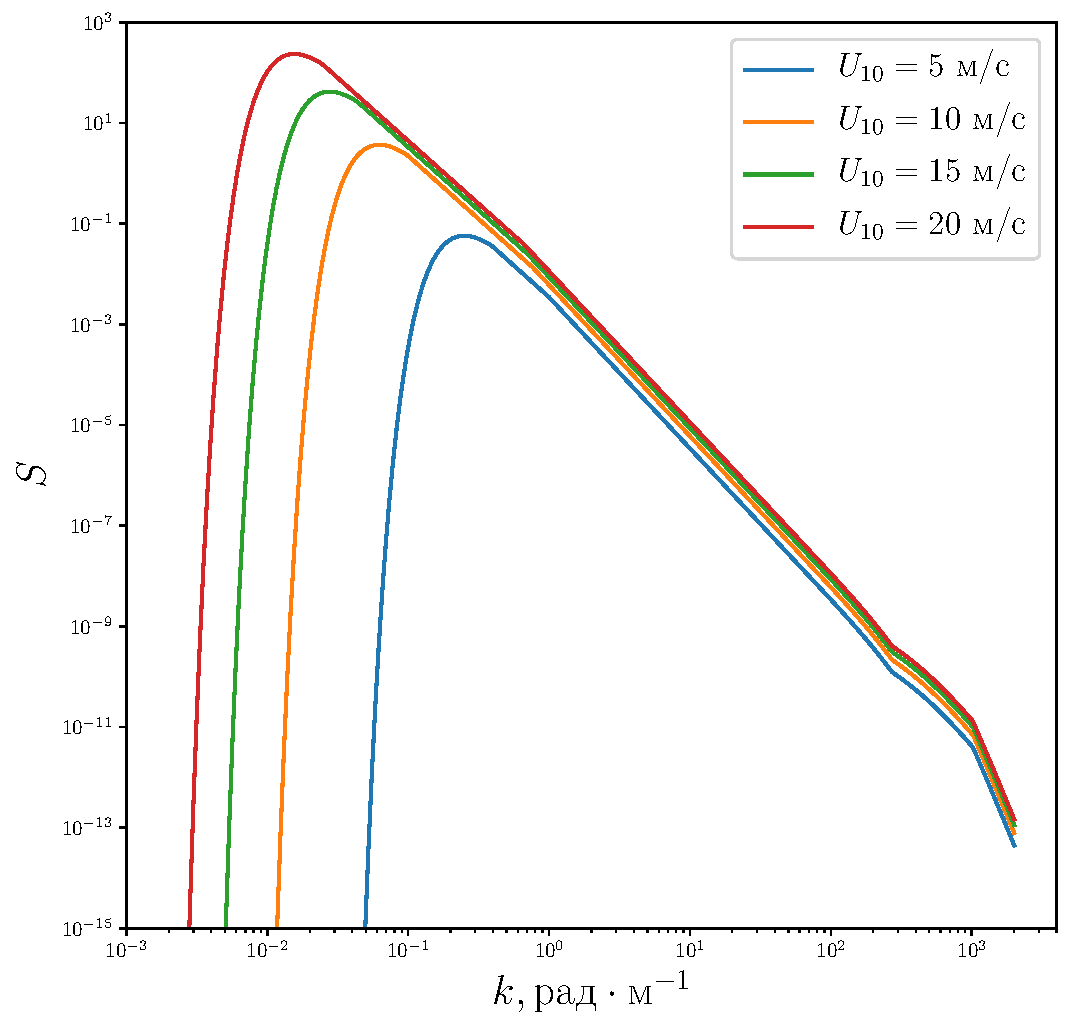
\includegraphics[width=0.6\linewidth]{fig/full_spectrum1}
        \caption{Спектр высот $S(k)$ при меняющейся скорости ветра}
        \label{fig:spectrum_heights}
\end{figure}

Графики $S(k)$ и  $\Phi_\xi(k)$ для наглядности изображены на рис.
\ref{fig:spectrum_heights} и рис. \ref{fig:angles_distrib} соответственно.
Далее $k_m$ будет называться ордината максимума функции  $S(k)$. Стоит
заметить, что с ростом скорости ветра число используемых гармоник, необходимых
для получения одинакового качества моделирования,
возрастает. На рис. \ref{fig:water} изображены поверхности,
построенные по формуле \eqref{eq:surface2d}.

\begin{figure}[h!]
    \begin{minipage}{0.49\linewidth}
        \centering
        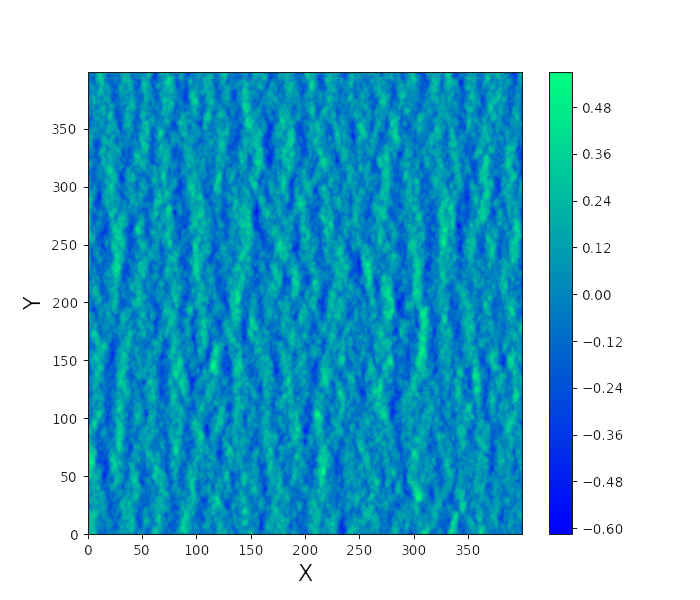
\includegraphics[width=\linewidth]{img/water5}

        (a)
    \end{minipage}
    \begin{minipage}{0.49\linewidth}
        \centering
        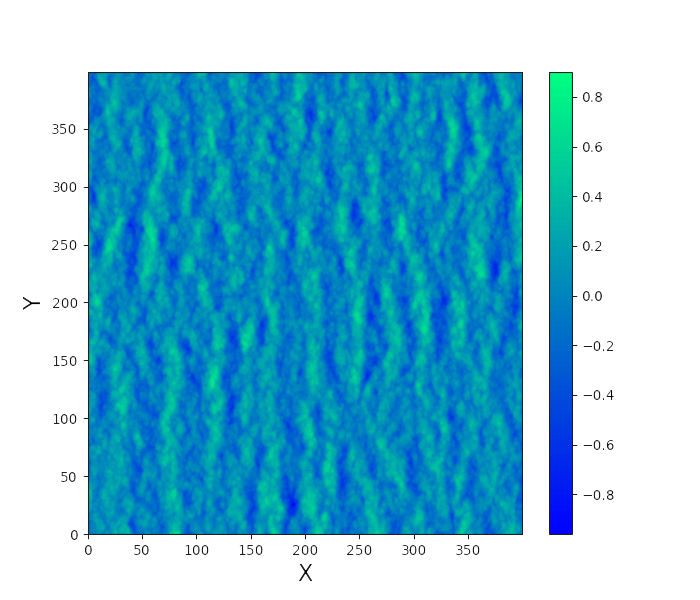
\includegraphics[width=\linewidth]{img/water6}

        (b)
    \end{minipage}
    \begin{minipage}{0.49\linewidth}
        \centering
        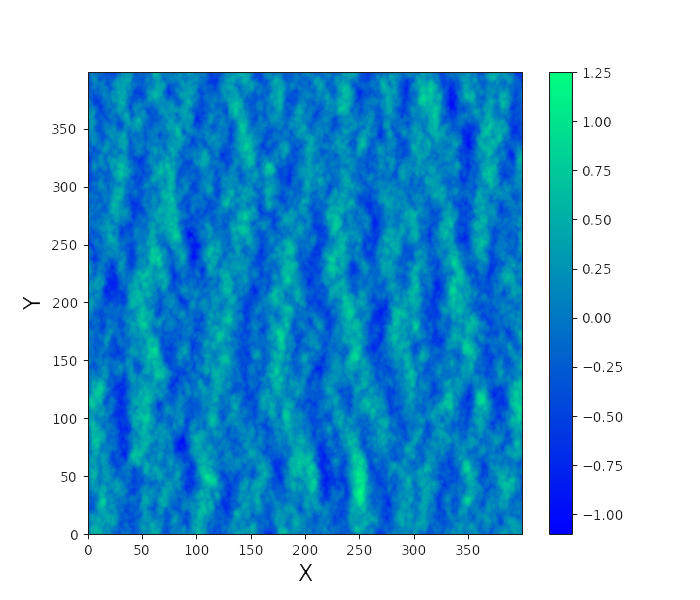
\includegraphics[width=\linewidth]{img/water7}

        (c)
    \end{minipage}
    \begin{minipage}{0.49\linewidth}
        \centering
        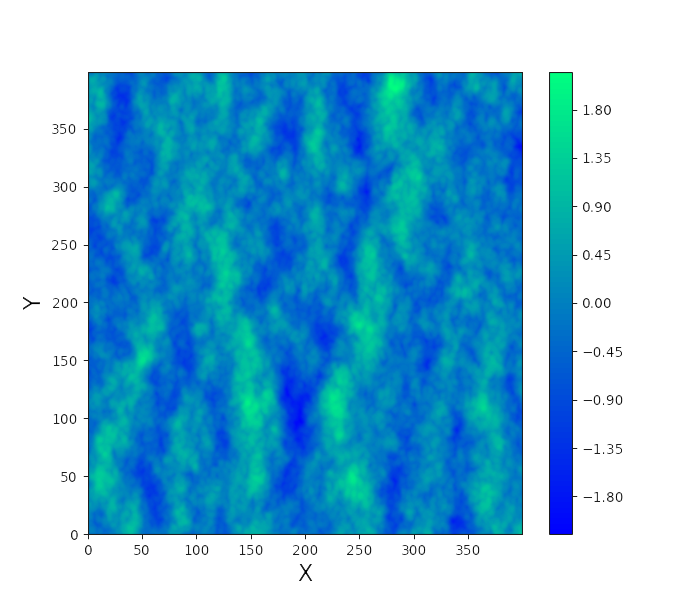
\includegraphics[width=\linewidth]{img/water10}

        (d)
    \end{minipage}
    \caption{Моделирование высот морского волнения: 
        (a) $U_{10} = 5 \text{м}/\text{c}$;
        (b) $U_{10} = 6 \text{м}/\text{c}$;
        (c) $U_{10} = 7 \text{м}/\text{c}$;
        (d) $U_{10} = 10 \text{м}/\text{c}$;
}
    \label{fig:water}
\end{figure}


Критерием качества моделирования, а также оптимального выбора числа гармоник
была выбранаблизость следующих корреляционных функций высот:
\begin{gather}
    \label{eq:KK}
    K[\rho] = \int\limits_{-\infty}^{\infty} S(k) \cos(k\rho) \dd k\\
    \tK(\rho) = \sum\limits_{n=1}^{N} \frac{A_n^2}{2} \cos(k_n \rho)
\end{gather}

\section{Метод <<отбеливания>> спектра.}%
\label{sec:metod_otbelivaniia_spektra_}

Для оптимизации времени построения поверхности и уменьшения количества гармоник
без уменьшения качества моделирования, предлагается использовать следующий
метод.

Предположим, что при больших $\rho$ гармонические составляющие корреляционной
функции не зависят друг от друга и мы можем пренебречь их взаимной корреляцией.
Тогда мощность <<шума>> функции $\tK (\rho)$ определяется выражением
$\displaystyle \sigma^2_{\text{шум}} = \sum\limits_{n=1}^{N} \frac{1}{2}
\frac{A^2_i}{2} \equiv \sum\limits_{n=1}^{N} \frac{b_i^2}{2}$.

В областях малых $\rho$, напротив, гармоники должны сильно взаимодействовать и
соответствующая мощность равна  $\displaystyle \tK^2(0) =
\qty(\sum\limits_{n=1}^{N} b_i)^2$ (см. \eqref{eq:KK} ).
Образуем величину
\begin{equation}
    \label{eq:Q}
    Q = \frac{\sigma_{\text{шум}}^2}{\tK^2(0)},
\end{equation}
которая характеризует относительную мощность шумов. Минимум этой величины
находится путём рещения системы уравнений
\begin{gather}
    \pdv{Q}{b_i} = 0, \text{ для } i=1,2,\dots, N. \\
    \frac{b_i \qty( \sum\limits_{n=1}^{N} b_i )^2 - 2 \sum\limits_{n=1}^{N} b_i
    \sum\limits_{n=1}^{N}  \frac{b_i^2}{2}}{\qty(\sum\limits_{n=1}^{N}
b_i)^4}=0
\end{gather}

Частным результатом её решения является $b_1 = b_2 = \dots = b_N$.

Спектр модельного поля при этом имеет близкий к белому вид, а выравнивание
амплитуд спектральных компонент поля $S(k)$ сводится к разбиению области
определения спектра $[k_{min},k_{max}]$ на участки $\Delta k_i$, интегралы по
которым от функции  $S(k)$ имеют одно и тоже значение $b_i = b_{0} =
\frac{\sigma^2}{N}$.

Заметим теперь, что рассуждая о способах разбиения интервала частот $[k_{min},
k_{max}]$ на участки $\Delta k_i$ мы оставляли нерешенным вопрос о выборе
расположения гармоник $k_i$ внутри этих участков. Обычно  $k_i$ ставится у
правой границы ячейки  $\Delta k_i$. При этом, однако, оказывается, что
модельная корреляционная функция плохо совпадает с экспериментальной
корреляционной функцией в области малых  $\rho$. Для достижения лучшего
согласия следует потребовать сопряжения всех производных (от первого до $N$-го
порядка) функций $\tK[\rho]$ и  $K[\rho]$ при  $\rho=0$. 
Поскольку $K'[\rho] = \pdv[2]{K[\rho]}{\rho}$, это условие эквивалентно
требованию сопряжения моментов спектро модельного и реального полей, которое
записывается в виде
 \begin{equation}
    \label{eq:}
    \sum\limits_{n=1}^{N} b_i k_i^{2p} 
    = \int\limits_{0}^{\infty} k^{2p}S(k) \dd k, 
\end{equation}

Полученная система $N$ уравнений для $N$ неизвестных $k_i$ не имеет общего
решения и потому может анализироваться лишь численно. Чтобы упростить решение
нашей задачи, потребуем облегченного, по сравнению с предыдущим, условия
сопряжения вторых моментов модельного и реального спектров высот
 \begin{equation}
    \label{eq:}
    b_i k_i^2 = \int\limits_{\Delta k_i} k^2 S(k) \dd k,
\end{equation}
где $b_i= A_i^2 / 2$

Из него непосредственно следует правило нахождения узлов $k_i$ 
\begin{equation}
    \label{eq:ki}
    \boxed{
        k_i = \sqrt{\frac{2}{A_{i}^2}} \int\limits_{\Delta k_i} k^2 S(k) \dd k. 
    }
\end{equation}

Формула \eqref{eq:ki} выведена для спектра высот поверхностного волнения. Когда
возникает необходимость моделирования уклонов, то необходима сделать замену
переменной $S(k) \to k^2 S(k)$, чтобы получить формулу для нахождения правила
расположения гармоник для уклонов

\begin{equation}
    \label{eq:ki_slopes}
    \boxed{
        k_i = \sqrt{\frac{2}{A_{i}^2}} \int\limits_{\Delta k_i} k^4 S(k) \dd k. 
    }
\end{equation}

\begin{figure}[h!]
    \centering
    \begin{minipage}{0.49\linewidth}
    \centering
    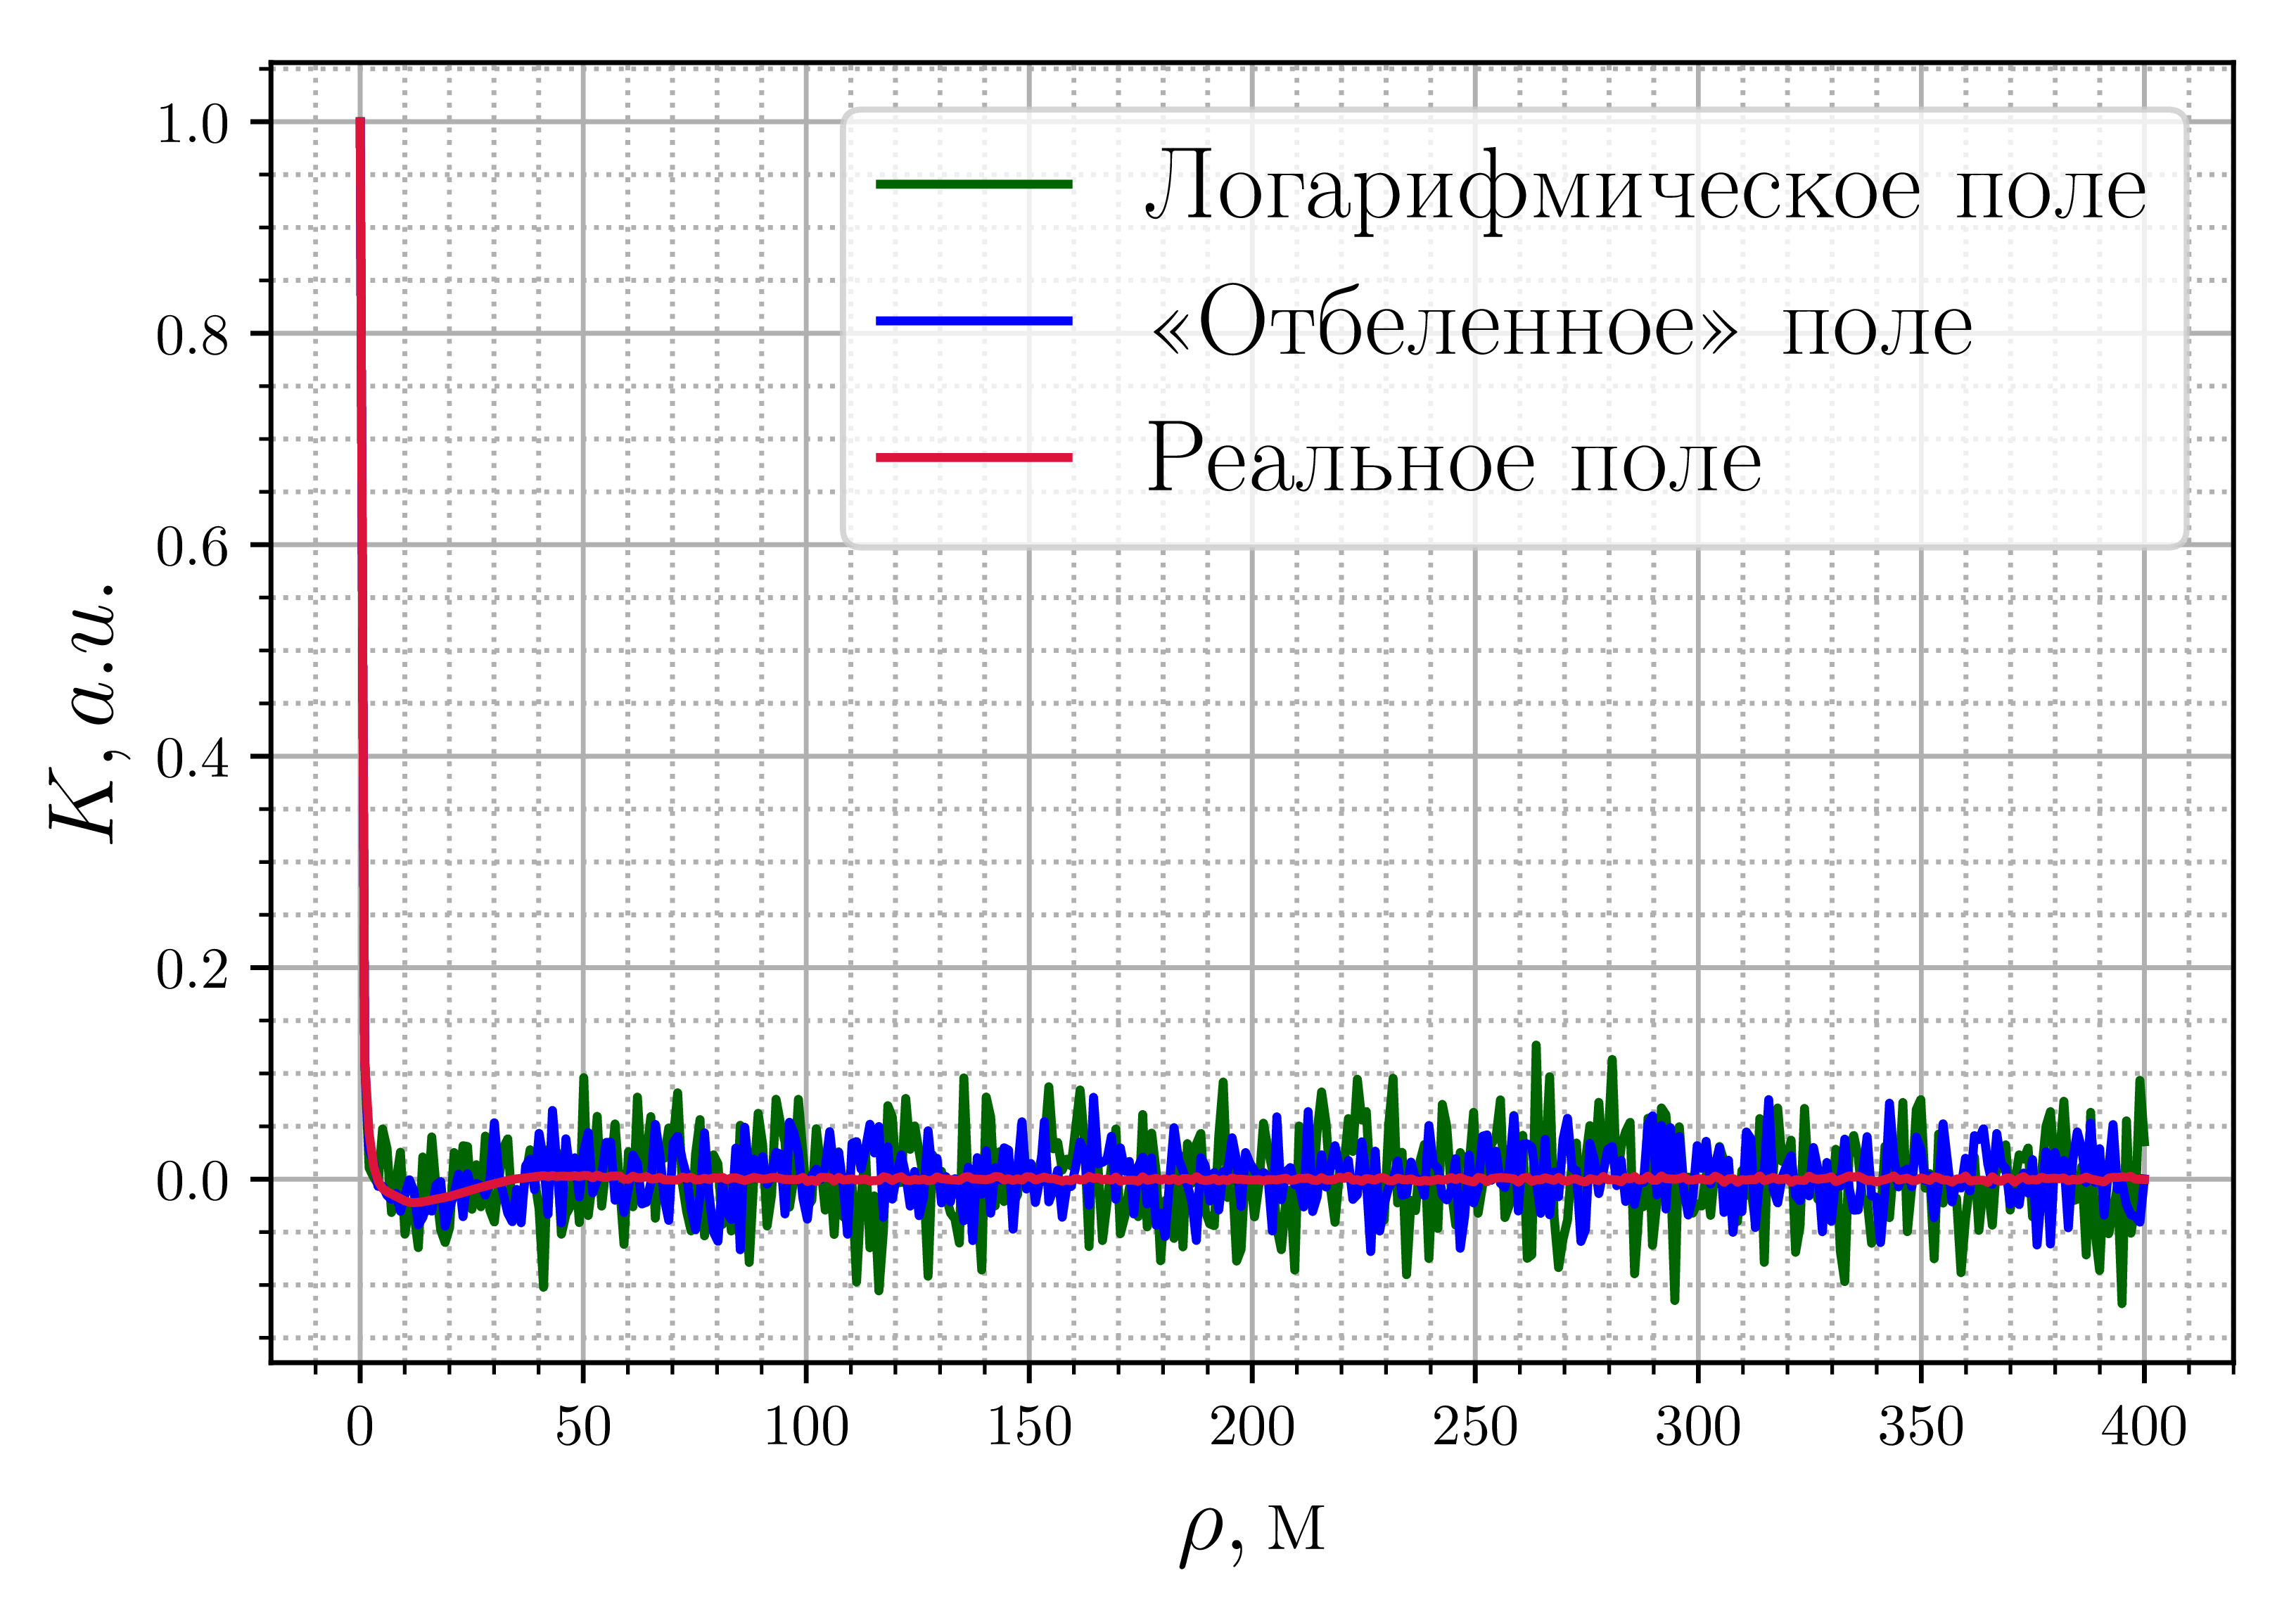
\includegraphics[width=\linewidth]{fig/correlation_angles_wa}

        (a)
    \end{minipage}
    \begin{minipage}{0.49\linewidth}
        \centering
        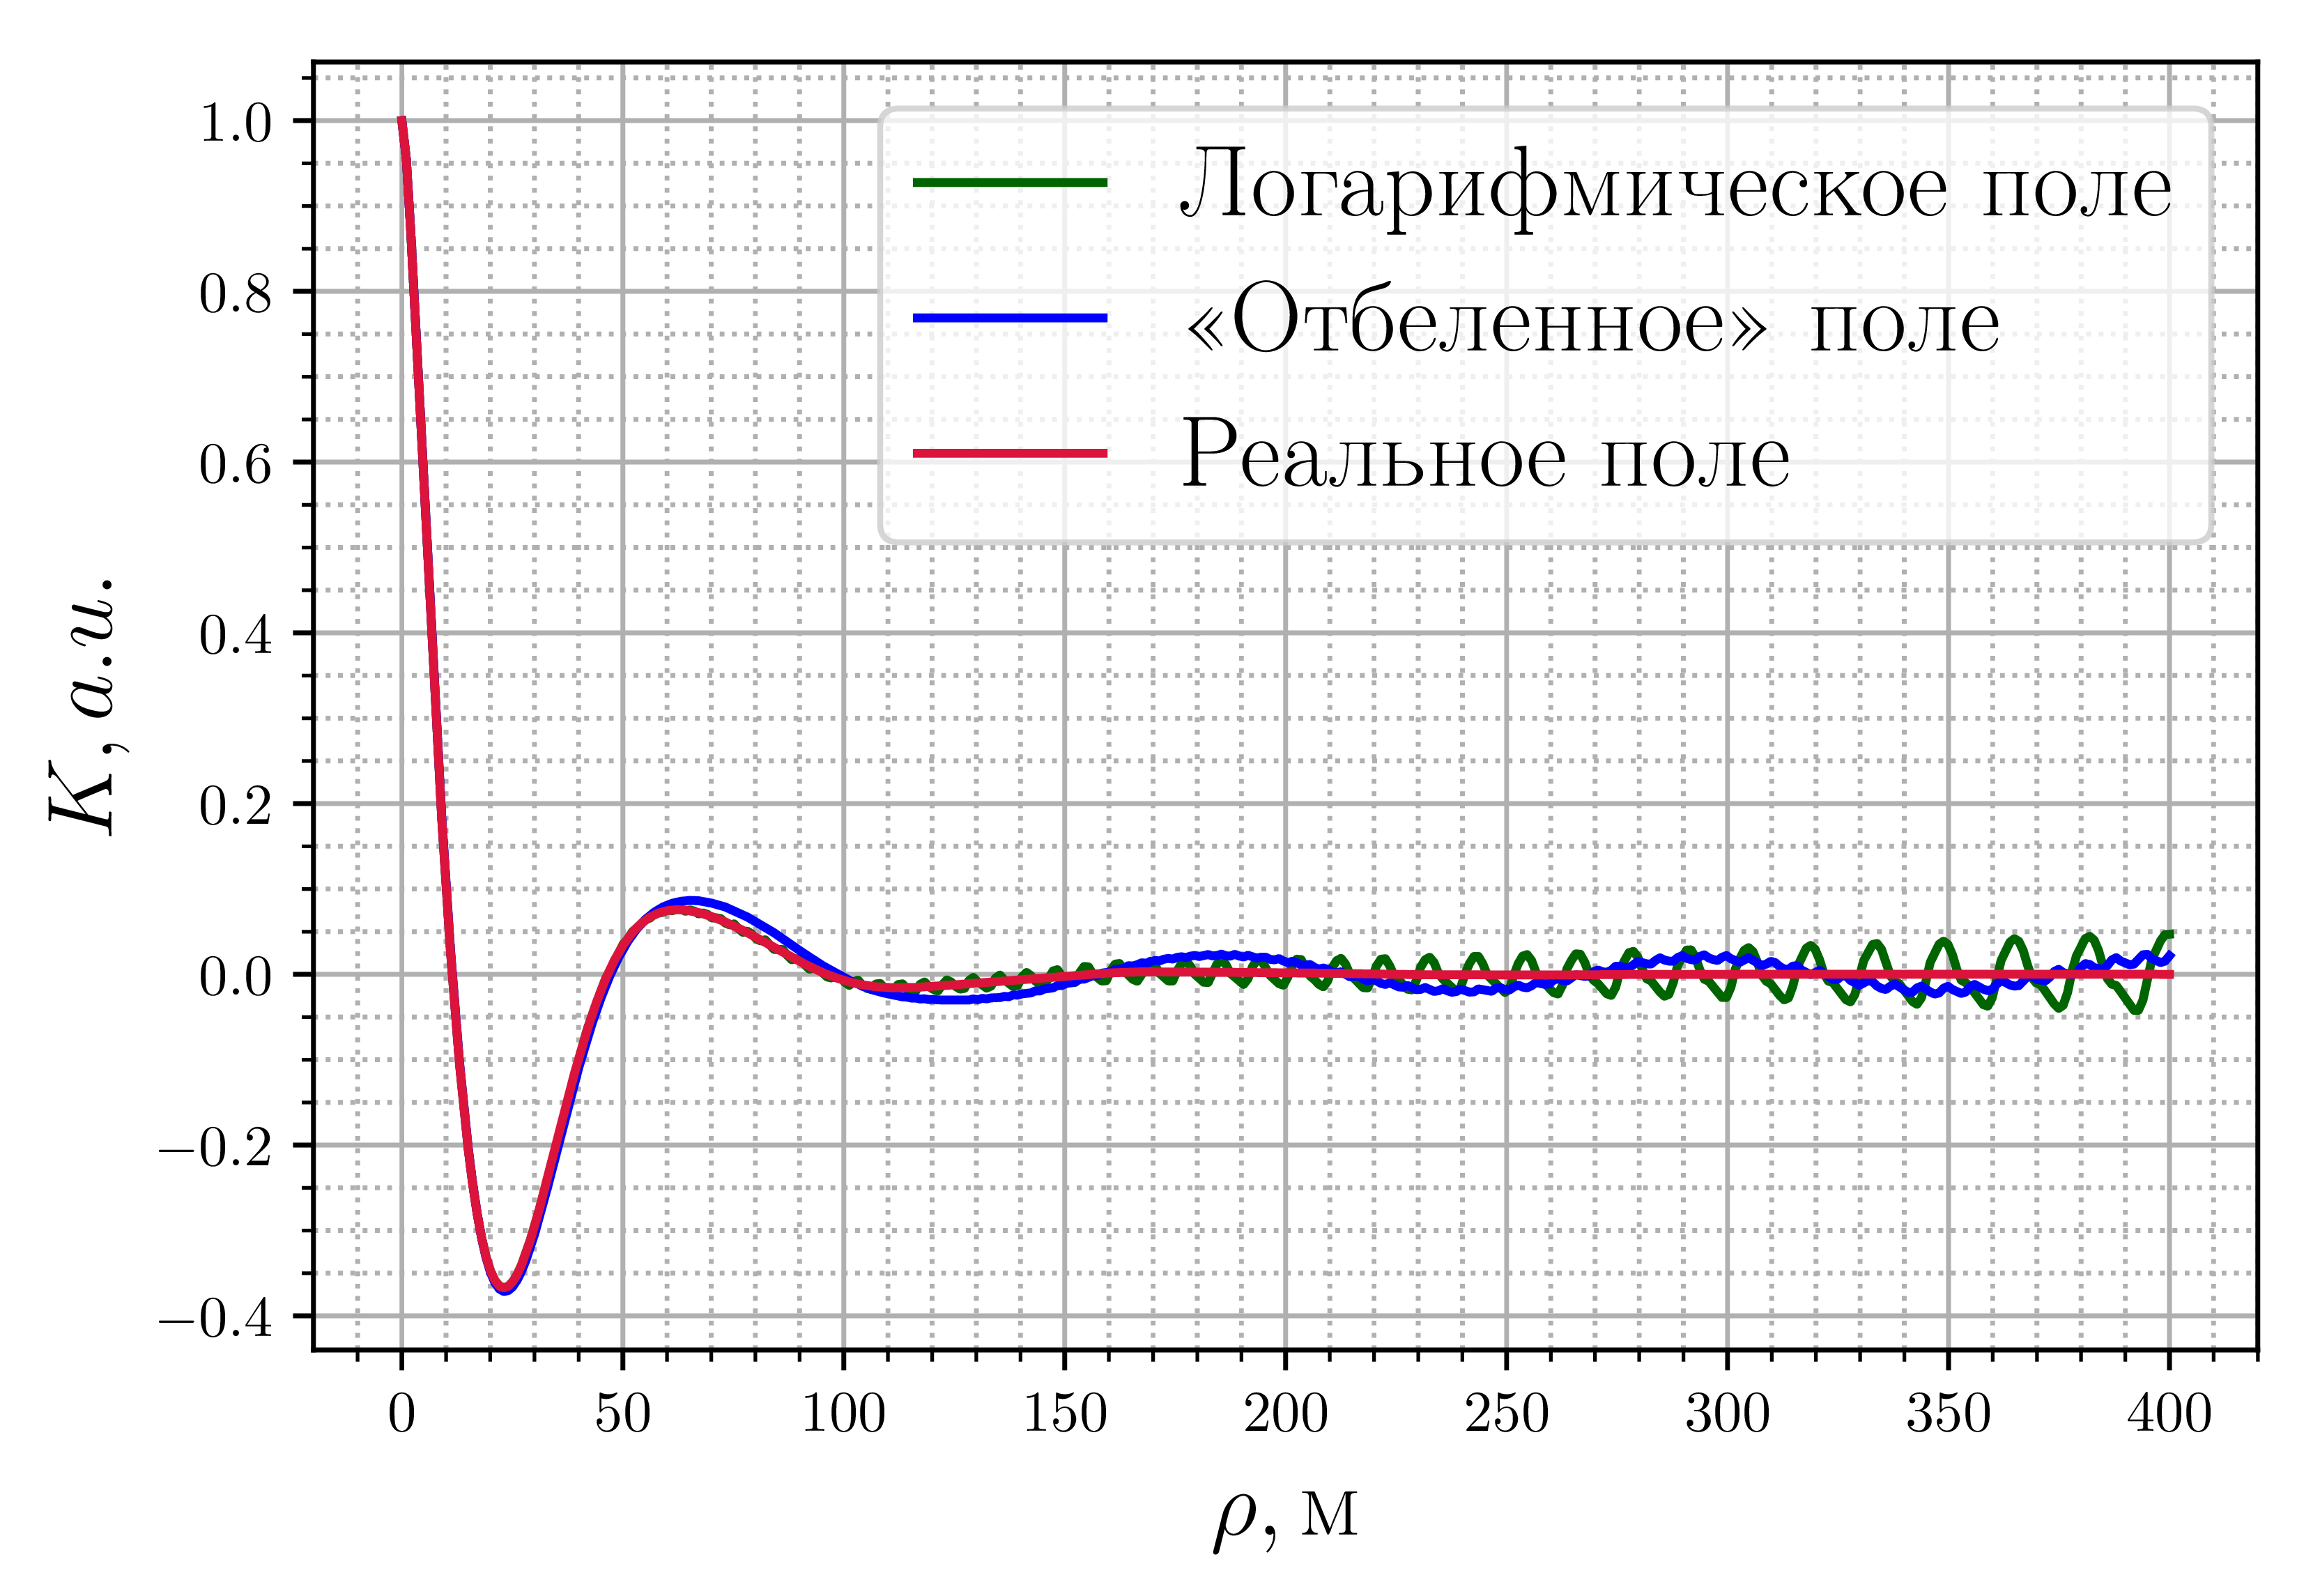
\includegraphics[width=\linewidth]{fig/correlation_height_wa}

        (b)
    \end{minipage}
    \caption{ Расположение гармоник по методу <<отбеливания>> спектра для
    наклонов и высот соответственно. }
    \label{fig:nodes}
\end{figure}

Такой способ выбора расположения гармоник, как нетрудно убедиться, обеспечивает
сопряжение корреляционных функций реального и модельного полей по второй
производной в нуле, или, иначе говоря, равенство дисперсий кривизн этих
полей.

\begin{figure}[h!]
    \centering
    \begin{minipage}{0.49\linewidth}
        \centering
        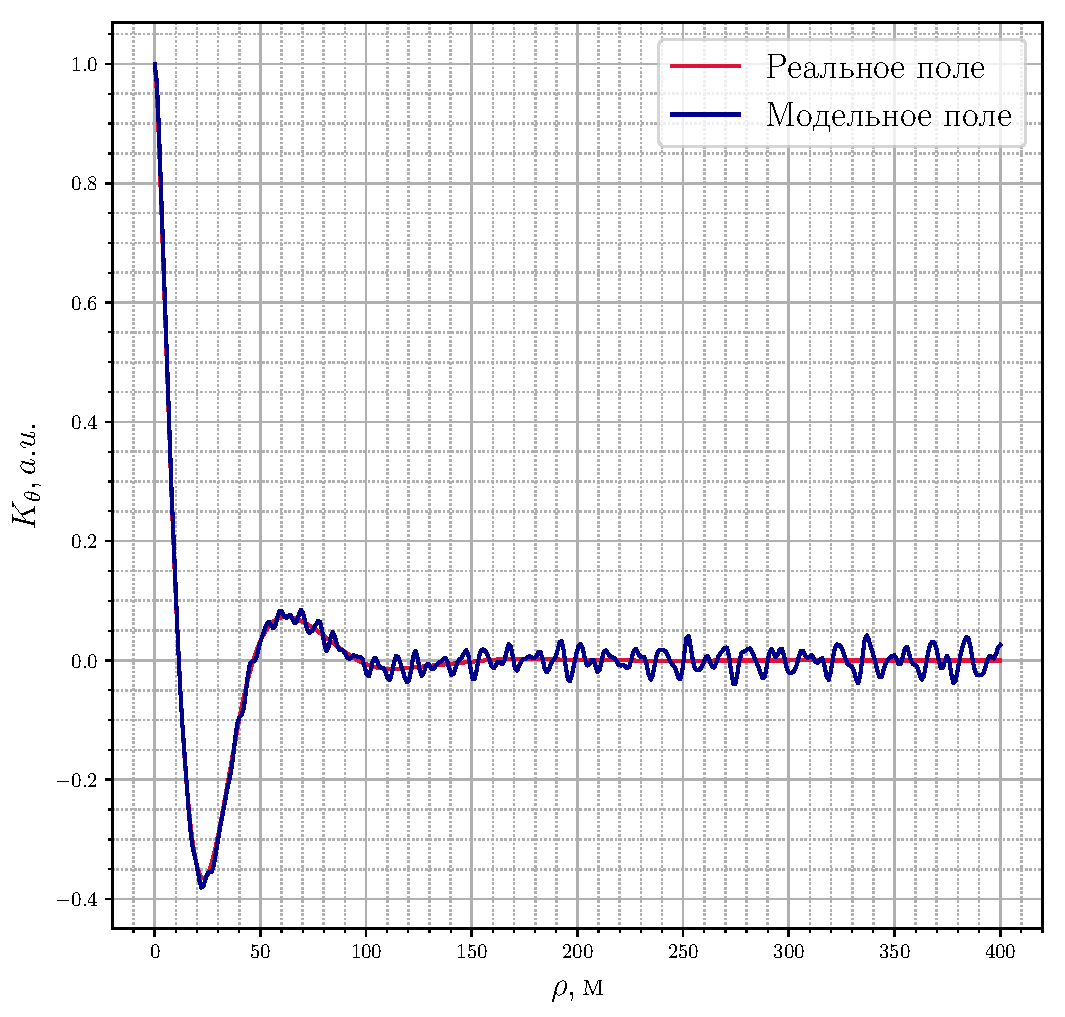
\includegraphics[width=\linewidth]{fig/correlation_height_height2}


        (a)
    \end{minipage}
    \begin{minipage}{0.49\linewidth}
        \centering
        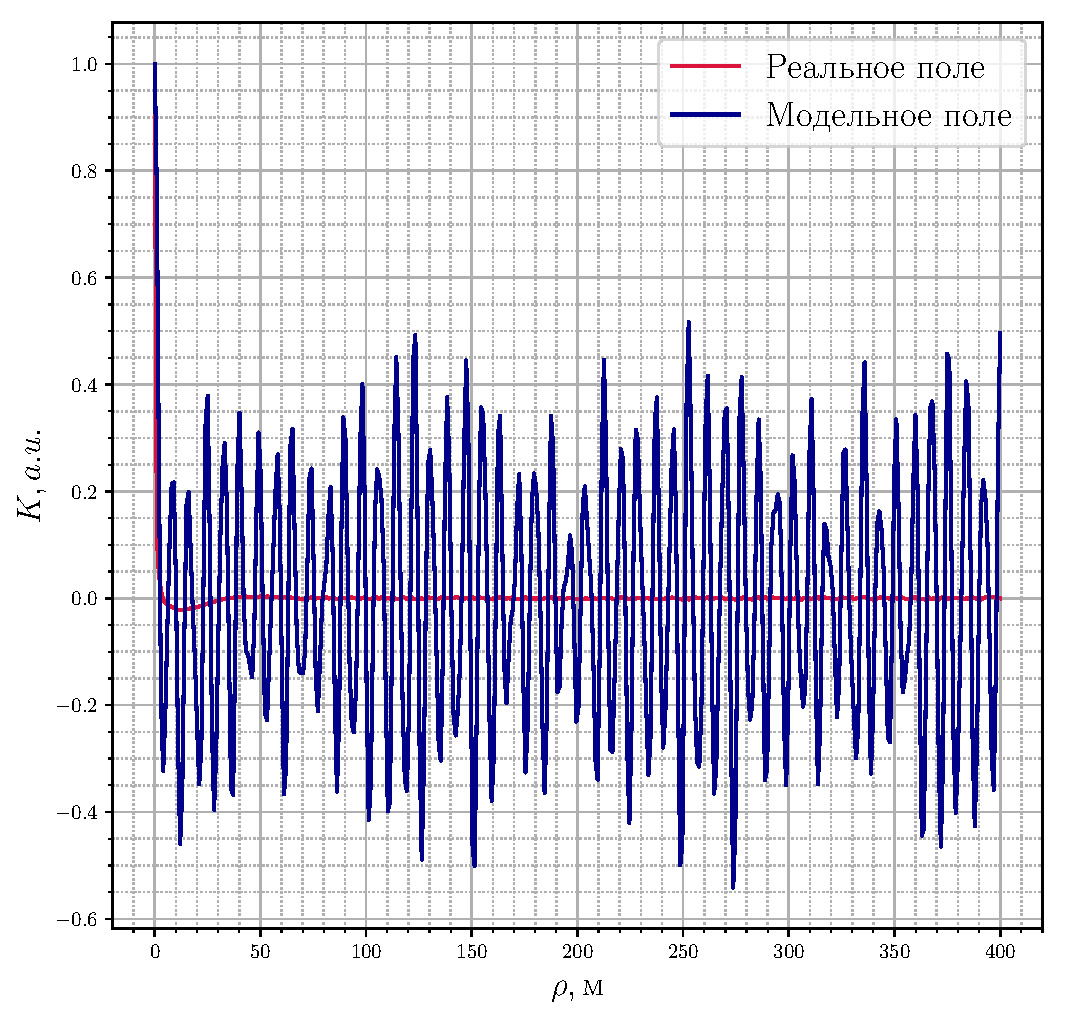
\includegraphics[width=\linewidth]{fig/correlation_angles_height2}



        (b)
    \end{minipage}

    \caption{ Корреляционные функции высот (a) и уклонов (b) при расположении гармоник
    по методу <<отбеливания>> спектра по формуле \eqref{eq:ki} }
    \label{fig:ki}
\end{figure}

\begin{figure}[h!]
    \centering
    \begin{minipage}{0.49\linewidth}
        \centering
        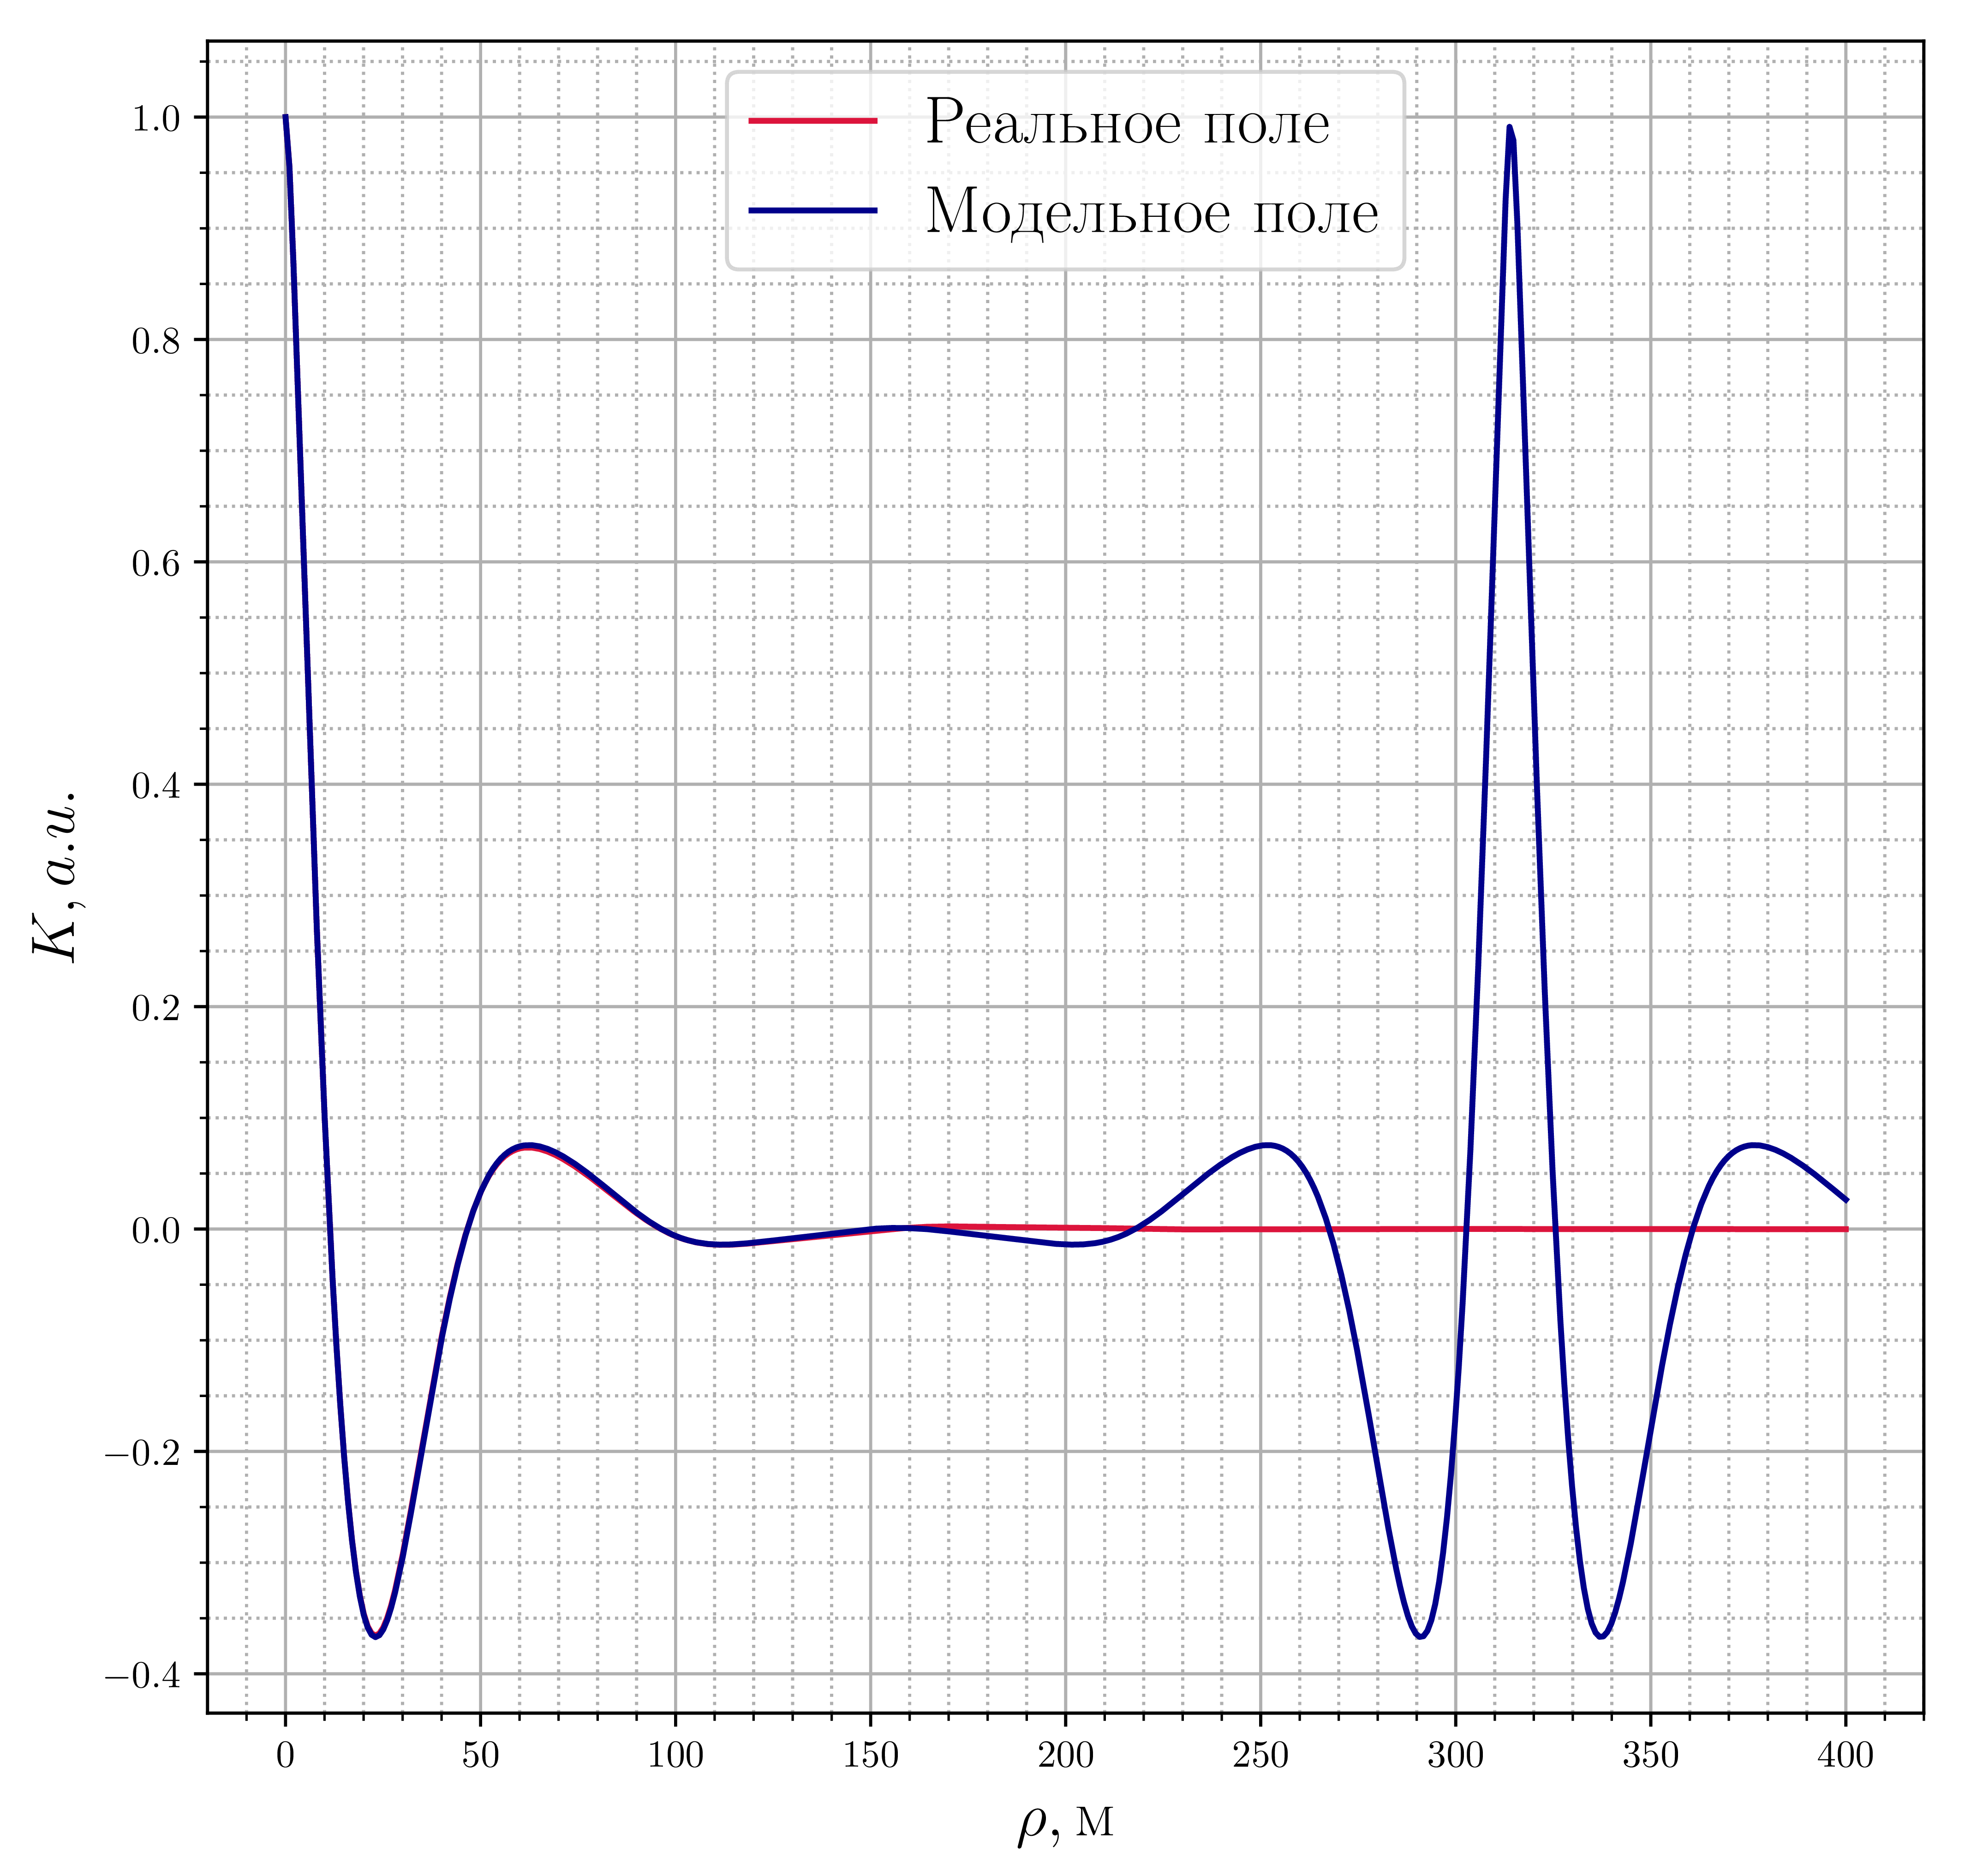
\includegraphics[width=\linewidth]{fig/correlation_height5_slopes2}

        (a)
    \end{minipage}
    \begin{minipage}{0.49\linewidth}
        \centering
        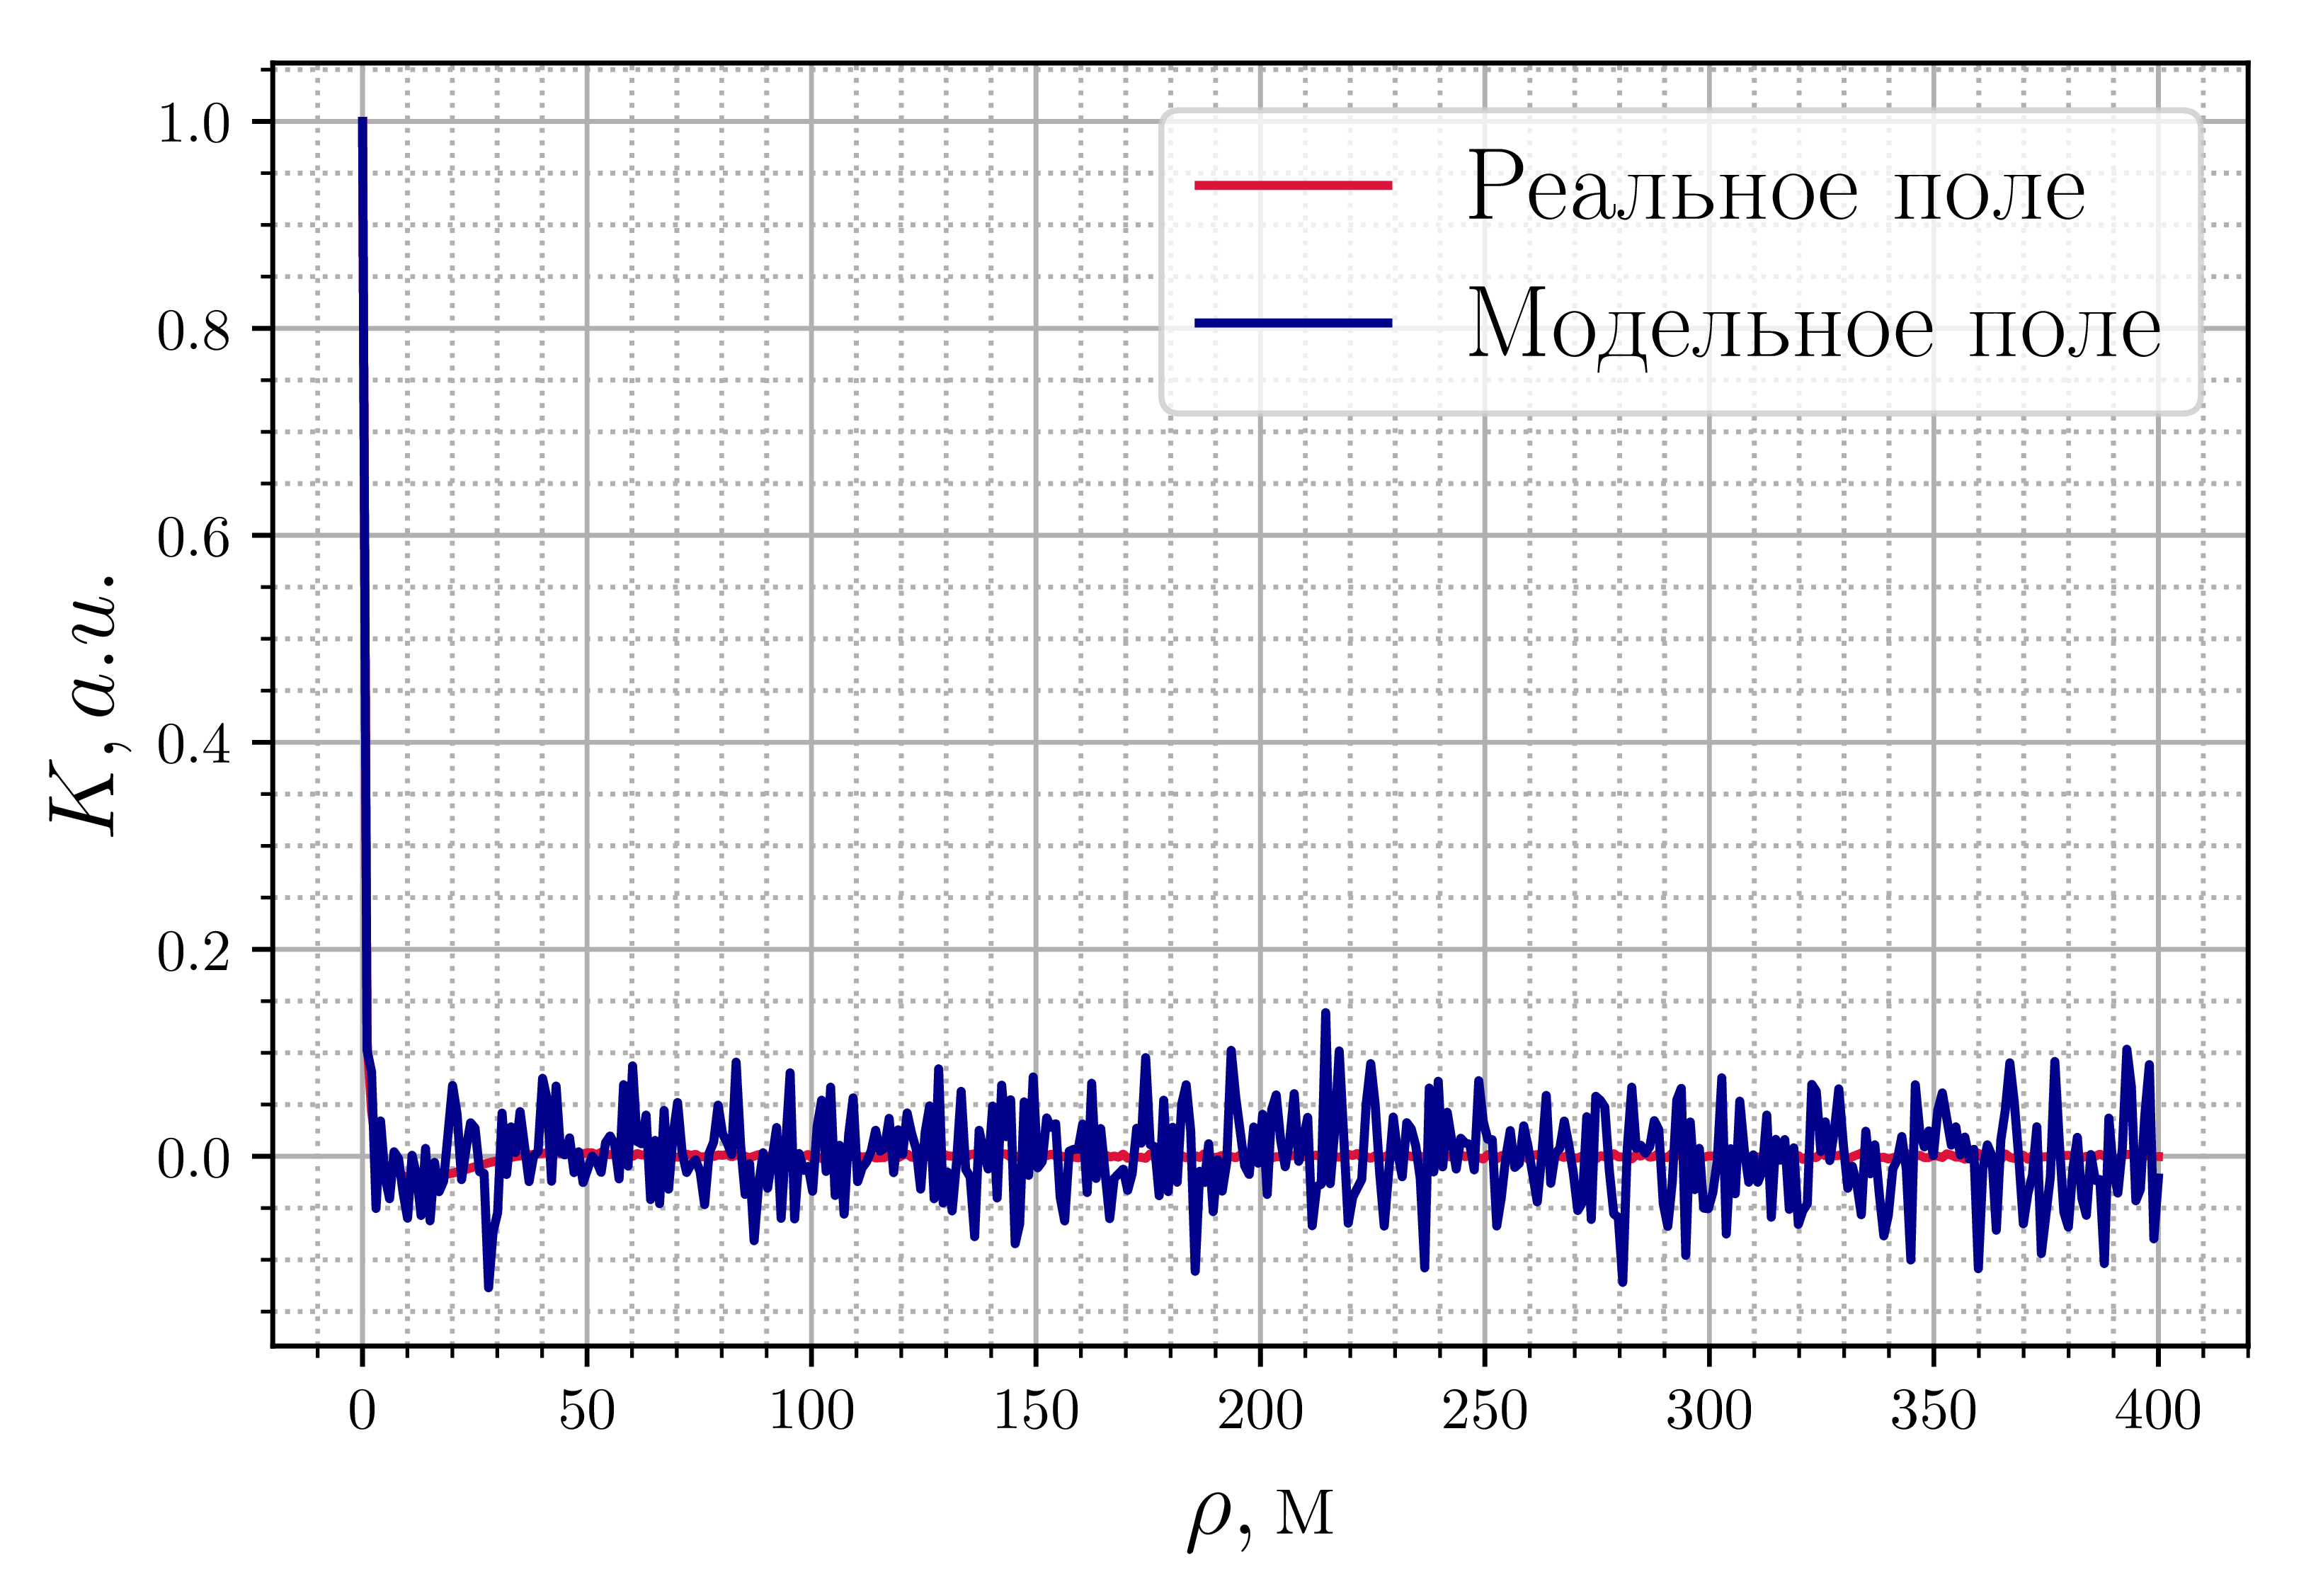
\includegraphics[width=\linewidth]{fig/correlation_angles_slopes2}

        (b)


    \end{minipage}
    \caption{ Корреляционные функции высот (a) и уклонов (b) при расположении гармоник
    по методу <<отбеливания>> спектра по формуле \eqref{eq:ki_slopes} }
    \label{fig:ki_slopes}
\end{figure}

Из рис. \ref{fig:ki} и \ref{fig:ki_slopes} видно, что нельзя такой метод, если
задача требует одновременного точного моделирования высот и уклонов
поверхности. 

Для такой задачи необходима рассмотреть другую функцию
относительных шумов $Q$, например
\begin{equation}
    \label{eq:Q_modif}
    Q = \frac{\qty(\sigma^{\text{н}}_{\text{шум}})^2}{(\tK^\text{н}(0))^2}+
        \frac{\qty(\sigma^{\text{в}}_{\text{шум}})^2}{(\tK^\text{в}(0))^2},
\end{equation}
где индексы <<н>> и <<в>> соответствуют наклонам и высотам. Учитывая то, что
оба слагаемых в уравнении \eqref{eq:Q_modif} вещественны и положительны, то 
экстремум функции $Q$ можно найти, зная экстремум каждого слагаемого по отдельности. 





\section{Choppy Wave Model}
\subsection{Обычный CWM}%

Рассмотрим задачу моделирования одномерной поверхности суммой гармоник 
 с детерменированными амплитудами и случайными фазами
 \begin{equation}
     \label{eq:}
     z = \sum\limits_{j=0}^{N} A_j \cos(k_j x + \psi_j)
 \end{equation}

Чтобы получить модель заостренной волны введем нелинейное преобразование координат
\begin{equation}
    \label{eq:}
    \qty{x,z(x)} \longrightarrow \qty{x + D(x),z(x)},
\end{equation}
где $D(x)$ горизонтальное смещение
\begin{equation}
    \label{eq:}
    D(x) =  \frac{i}{2\pi} \int\limits_{-\infty}^{\infty}   S(k) e^{ikx} \dd{k},
\end{equation}
а $S(k)$ -- прямое Фурье преобразование исходной поверхности
\begin{equation}
    \label{eq:}
    S(k) = \int\limits_{-\infty}^{\infty} z(x) e^{-ikx} \dd x 
\end{equation}

В нашем случае, функция $D(x)$ примет вид: 
\begin{equation}
    \label{eq:}
    \begin{cases}
    x = x_{0} \underbrace{
    - \sum\limits_{j=0}^{N} A_j \sin(k_j x_0 + \psi_j)
    }_{D(x)} \\
        z = \sum\limits_{j=0}^{N} \cos(k_j x_{0} + \psi_j)
    \end{cases}
\end{equation}
Это и есть Choppy Wave Model. График подобной заостренной поверхности 
изображен на рис.\ref{fig:1}


Рассчитаем спектр  поверхности, построенной по CWM.

 Спектр поверхности в новых координатах 
 \begin{equation}
     \label{eq:S_cwm}
     \widehat S(k) = \int\limits_{-\infty}^{\infty} z(x) \cdot  
     e^{-ikx} \qty[ 1 + D'(x)]
     \dd{x}  = S(k) + \int\limits_{-\infty}^{\infty} z(x) \cdot D'(x)  
     e^{-ikx}\dd{x},
 \end{equation}

 где $S(k)$-- исходный спектр (например, JONSWAP).

 Пусть спектр $S(k)$ состоит из всего одной гармоники. Тогда, мы можем его
 записать в виде
 \begin{equation}
     \label{eq:}
     S(k) = \pi A_{0}( \delta(k-k_{0}) + \delta(k+k_{0}))
 \end{equation}

 Для такого спектра функция горизонтального смещения и её производная равны:
 \begin{equation}
     \label{eq:}
     D(x) = -A_{0} \sin(k_{0} x), \quad
     D'(x) = -A_{0} k_{0} \cos(k_{0} x)
 \end{equation}

 Запишем прямое преобразование Фурье для функции $D'(x)$:
 \newcommand{\D}{\mathfrak{D}}
  \begin{equation}
     \label{eq:}
     \D(k) = \int\limits_{-\infty}^{\infty} D'(x) e^{-ikx} \dd x =
     - \pi A_{0}k_{0}\qty[\delta(k-k_{0})+\delta(k+k_{0})]
 \end{equation}

 Перепишем \eqref{eq:S_cwm}, применяя теорему о свертке:
\begin{equation}
    \label{eq:}
    \widehat S(k) = S(k) +
    \frac{1}{2\pi} \int\limits_{-\infty}^{\infty} S(k-\xi) \D(\xi) \dd \xi 
\end{equation}
\begin{gather}
    \label{eq:}
    \widehat S(k) = S(k) + \frac{A_{0}}{2} \qty[\D(k-k_{0}) + \D(k+k_{0})] = \\
    S(k) - \frac{\pi A_{0}^2}{2} k_{0} \qty[
    \delta(k-2k_{0}) +
    \delta(k+2k_{0}) +
    \delta(k) +
    \delta(k) 
    ] = \\
    \pi A_{0}[\delta(k+k_{0})+ \delta(k-k_{0})] -
    \frac{\pi A_{0}^2k_{0}}{2}\qty[ \delta(k+2k_{0}) + 2\delta(k) +
    \delta(k-2k_{0})]
\end{gather}
Итак, для частного случае, когда моделируемая поверхность представляет всего
одну гармонику $z(x) = A_{0}\cos(k_{0}x)$
Мы получили модифицированный спектр:
\begin{equation}
    \label{eq:}
    \widehat S = 
    \pi A_{0}[\delta(k+k_{0})+ \delta(k-k_{0})] -
    \frac{\pi A_{0}^2k_{0}}{2}\qty[ \delta(k+2k_{0}) + 2\delta(k) +
    \delta(k-2k_{0})]
\end{equation}

Очевидно, что если поверхность будет представляться суммой гармоник
$z(x) = \sum\limits_{n=0}^{N} A_n \cos{k_n x}$,
спектр примет вид
\begin{equation}
    \label{eq:}
    \widehat S = 
    \underbrace{
    \sum\limits_{n=0}^{N} \pi A_n \qty[\delta(k+k_n) + \delta(k-k_n) ]
}_{S(k)}
\underbrace{
- \sum\limits_{n=0}^{N} \frac{\pi A_{n}^2 k_n}{2}
\qty[ \delta(k+2k_{n}) 
    + 2\delta(k) 
+ \delta(k-2k_{n})]
}_{S_{CWM}(k)}
\end{equation}

Добавка к исходному спектру выглядит следующим образом
\begin{gather}
    \label{eq:}
    \boxed{
    S_{CWM}(k) = - \sum\limits_{n=0}^{N} \pi A_{n}^2 k_n \delta(k) - 
    \sum\limits_{n=0}^{N} \frac{\pi A_n^2 k_n}{2} \qty[\delta(k+2k_n) +
    \delta(k-2k_n)]
}
\end{gather}

\begin{figure}[H]
    \begin{minipage}{0.49\linewidth}
        \centering
        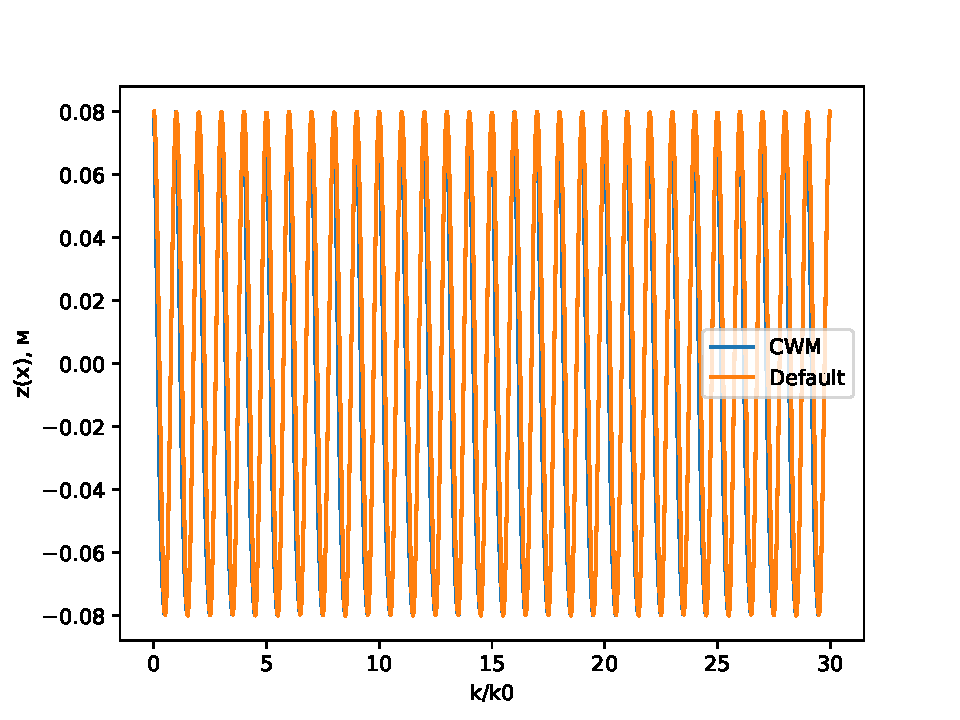
\includegraphics[width=\linewidth]{fig/cwm_surface.pdf}

        (a)
        \caption{Заостренная синусоида (CWM) в сравнении обычной}
        \label{fig:1}
    \end{minipage}
    \hfill
    \begin{minipage}{0.49\linewidth}
        \centering
        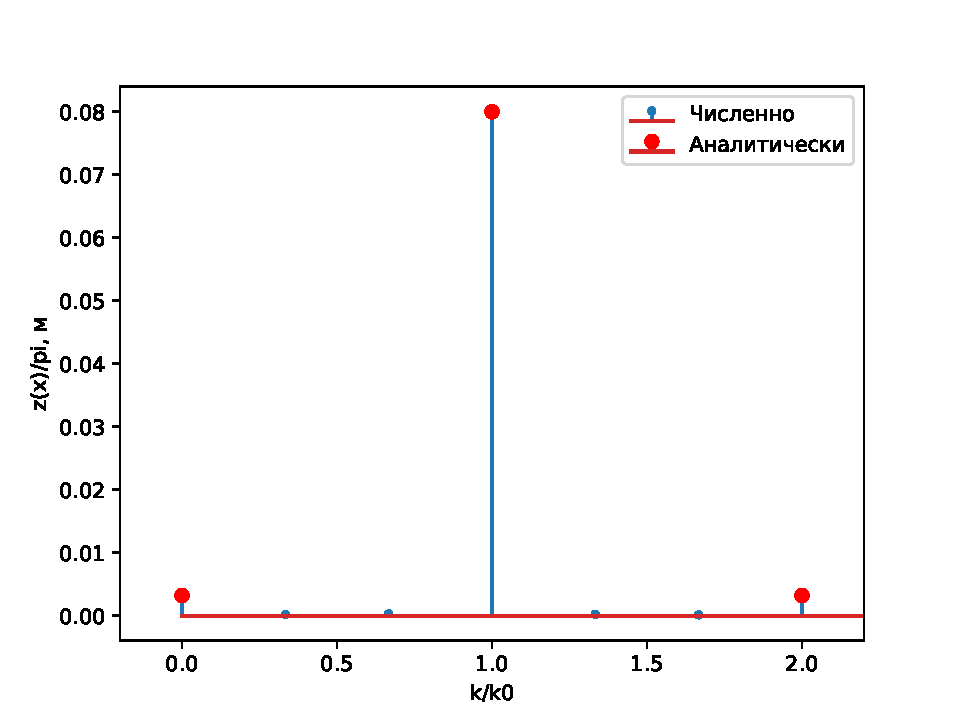
\includegraphics[width=\linewidth]{fig/cwm_spectrum.pdf}

        (b)
        \caption{Спектр заостренной синусоиды}
        \label{fig:2}
    \end{minipage}

\end{figure}
 \subsection{Модифицированный CWM}%
 
 Для того, чтобы получить ассиметричную, заостренную поверхности введем другую
 функцию горизонтального смещения
 $D(x)$
 \begin{equation}
     D(x) = 
     \begin{cases}
          - A_{0} \sin(k_{0}x), &\text{ если }  0 \leq k_{0} x \leq  \pi \\
         0, & \text{ если }  \pi < k_{0} x < 2 \pi
     \end{cases}
 \end{equation}
И снова введем преобразование координат
\begin{equation}
    \label{eq:}
    \qty{z(x),x} \to \qty{z(x), x + D(x)}
\end{equation}
 Спектр поверхности в новых координатах 
 \begin{equation}
     \label{eq:}
     \widehat S(k) = \int\limits_{-\infty}^{\infty} z(x) \cdot  
     e^{-ikx} \qty[ 1 + D'(x)]
     \dd{x}  = S(k) + \int\limits_{-\infty}^{\infty} z(x) \cdot D'(x)  
     e^{-ikx}\dd{x},
 \end{equation}
 где $S(k)$-- исходный спектр (например, JONSWAP).

%\begin{figure}[h!]
    %\begin{minipage}{0.45\linewidth}
        %\centering
        %\includegraphics[width=\linewidth]{example-image-a}
        %\caption{График функции $D(x)$}
    %\end{minipage}
    %\hfill
    %\begin{minipage}{0.45\linewidth}
        %\centering
        %\includegraphics[width=\linewidth]{example-image-a}
        %\caption{График функции $D'(x)$}
    %\end{minipage}
    %\label{fig:}
%\end{figure}

 Задача сводится теперь к вычислению интеграла
 \begin{equation}
     \label{eq:}
     I(k) = \int\limits_{-\infty}^{\infty} z(x) \cdot D'(x) e^{-ikx}\dd x 
 \end{equation}



Согласно теореме о свертке 
\begin{equation}
    \label{eq:I}
    I(k) = \frac{1}{2\pi} \int\limits_{-\infty}^{\infty}  S(k-\xi) \D(\xi)\dd{\xi}, \text{ где}
\end{equation}
$\D(k) = \int\limits_{-\infty}^{\infty} D'(x) e^{-i k x}\dd{x} $,
$S(k) = \int\limits_{-\infty}^{\infty} z(x) e^{-i k x}\dd{x} $ --
обратное Фурье-преобразование функций $D'(x)$ и  $z(x)$ соответственно.
\subsubsection{Нахождение спектральной плотности функции $D'(x)$}%
Для простоты рассмотрим случай одной гармоники. 

В этом случае $D(x)$ можно представить в виде модуляции гармонического сигнала
прямоугольным сигналом.


$D(x)$ представим в виде произведения двух функций 
$D(x) = -A_{0}\sin(k_{0}x) \cdot  \Theta(k_{0} x)$,
где $\Theta(k_{0}x)$ -- прямоугольный сигнал.

Запишем прямое преобразование Фурье 
\begin{gather}
    \label{eq:D}
    \D(k) = \int\limits_{-\infty}^{\infty} D'(x) e^{-ikx} \dd{x} = \\
    - A_0 k_0\int\limits_{-\infty}^{\infty} 
     \cos k_{0}x\cdot \Theta (k_{0} x) e^{-ikx}\dd x
     - A_{0}
     \underbrace{
     \int\limits_{-\infty}^{\infty} 
    \Theta'(k_{0} x) \sin(k_{0} x) e^{-ikx}\dd x
}_{=~0} = \\
    = \int\limits_{-\infty}^{\infty} 
    \underbrace{- A_{0} k_{0} \cos k_{0}x\cdot}_{f(x)}
    \underbrace{\Theta (k_{0} x) }_{g(x)}e^{-ikx}
    \dd x = \int\limits_{-\infty}^{\infty} f(x) g(x) e^{-ikx} \dd x. 
\end{gather}
Осталось найти спектр функций $f(x)$ и  $g(x)$ и снова воспользоваться теоремой о свертке.

\paragraph{Спектр функции $f(x)$.}%
\begin{gather}
    S_f(k) = - A_{0} k_{0}\int\limits_{-\infty}^{\infty} \frac{e^{+ik_{0}x} + e^{-ik_{0}x}}{2} e^{-ikx} \dd x = \\ 
    - \frac{A_{0} k_{0}}{2}
    \underbrace{ 
         \int\limits_{-\infty}^{\infty} e^{-i(k-k_{0})x}\dd{x}  
    }_{2 \pi \delta(k-k_{0})}
    - \frac{A_{0} k_{0}}{2} 
    \underbrace{
    \int\limits_{-\infty}^{\infty} e^{-i(k-k_{0})x}\dd{x} 
    }_{2 \pi \delta(k+k_{0})} = \\
    -\frac{A_{0} k_{0}}{2} \cdot 2 \pi \qty{ \delta(k-k_{0}) + \delta(k+k_{0}) } = \\
    \boxed{
    - \pi A_{0} k_{0} \qty{ \delta(k-k_{0}) + \delta(k+k_{0})}
    }
\end{gather}

\paragraph{Спектр функции $g(x)$.}%
$X = \frac{2\pi}{k_{0}}$ -- период прямоугольного импульса, совпадающий с
периодом синусоиды частотой 
$k_0$. При этом $k_n = n k_0$
\newcommand{\sinc}[1]{\textrm{sinc}\qty(#1)}
\begin{gather}
    C_n(k) = \frac{1}{X} \int\limits_{0}^{\frac{X}{2}} e^{-i k_n x} \dd{x} = 
    \frac{1}{- i k_n X} e^{-i k_n x} \eval_{0}^{\frac{X}{2}} =
    \frac{1}{- i k_n X} \qty( e^{-i \frac{k_n X}{2}} - 1) = \\
    \frac{1}{- i k_n X} e^{-i \frac{k_n X}{4}}\qty( e^{-i \frac{k_n X}{4}} - e^{+i \frac{k_n X}{4}}) = \frac{e^{-i \frac{k_n X}{4}}}{2} \cdot \sinc{\frac{k_n X}{4}}
\end{gather}

\begin{gather}
    \label{eq:G}
    S_g(k) =\frac{e^{-i  \frac{\pi}{2 k_0}  k} }{2}\cdot
    \sinc{\frac{\pi}{2k_{0}}k}\sum\limits_{n=-\infty}^{\infty}  2 \pi\delta(k - n
    k_0)
\end{gather}

Вернемся к \eqref{eq:D} 
\begin{equation}
    \label{eq:}
    \D(k) = \frac{1}{2 \pi} \int\limits_{-\infty}^{\infty} S_f(k-x) S_g(x)
    \dd{x} = - \frac{A_{0} k_{0}}{2} \qty[S_g(k-k_{0}) + S_g(k+k_{0})].
\end{equation}
Переобозначим $\D_{\pm}(k) = - \frac{A_{0} k_{0}}{2} S_g(k \mp k_{0})$.
Распишем теперь эту формулу, используя \eqref{eq:G}:
\begin{equation}
    \label{eq:}
    \D_{\pm} = -\frac{A_{0}k_{0}}{2} \cdot \frac{e^{-i  \frac{\pi}{2 k_0}
    (k\mp k_{0})} }{2}\cdot
    \sinc{\frac{\pi}{2k_{0}}(k\mp k_{0})}\sum\limits_{n=-\infty}^{\infty} 2\pi  \delta(k - n
    k_0)
\end{equation}

Вернемся теперь к уравнению \eqref{eq:I}. 
Для него мы нашли $\D(k)$.
в случае одной гармоники равен  $S(k) = \pi A_0 \qty{\delta(k-k_{0}) +
\delta(k+k_{0})}$.
Получаем


\begin{gather}
    I(k) = \frac{1}{2\pi} \int\limits_{-\infty}^{\infty}  S(k-\xi)
    \D(\xi)\dd{\xi} = \\
    \frac{1}{2\pi} \int\limits_{-\infty}^{\infty} \pi A_{0}\qty{
    \delta(\xi- (k-k_{0}) ) + \delta(\xi - (k+k_{0})) } 
    \cdot \qty{\D_{+}(\xi) + \D_{-}(\xi)} \dd \xi = \\
    \frac{A_{0}}{2} (
    \D_{+}(k-k_{0}) +
    \D_{+}(k+k_{0}) +
    \D_{-}(k+k_{0}) +
    \D_{-}(k-k_{0}) 
    ) = \\
    -\frac{A_{0}^2 k_{0}}{2} \qty[
    S_g(k-2k_{0}) +
    S_g(k+2k_{0}) +
    2S_g(k)
    ]
\end{gather}

\begin{equation}
    \boxed{
    \widehat S(k) = S(k)  
    -\frac{A_{0}^2 k_{0}}{2} \qty[
    S_g(k-2k_{0}) +
    S_g(k+2k_{0}) +
    2S_g(k)
    ] }
\end{equation}
\begin{equation}
\boxed{
    S_g(k) =\frac{e^{-i  \frac{\pi}{2 k_0}  k} }{2}\cdot
    \sinc{\frac{\pi}{2k_{0}}k}\sum\limits_{n=-\infty}^{\infty}  
    2 \pi\delta(k - n k_0)
}
\end{equation}

\appendix

\newpage
\section{Спектральное представление непериодических сигналов}%
Пусть $U(t)$ одиночный импульс конечной длительности. Создадим периодическую
последовательность с периодом $T$ и представим её комплексным рядом Фурье

\begin{equation}
    \label{eq:1}
    U_{\text{периодич} } (t) = \sum\limits_{n=-\infty}^{\infty} C_n \exp{ i n \omega_0 t},
\end{equation}
где 
\begin{equation}
    \label{eq:2}
    C_n =\frac{1}{T} \int\limits_{- \frac{T}{2}}^{\frac{T}{2}} U(t) \exp{-in\omega_{0}t } \dd t
\end{equation}

Для того, чтобы перейти к спектральному представлению единичного импульса,
устремим $T \to  \infty$.

Из \eqref{eq:2} видно, что при $T \to \infty$ получаем:
\begin{enumerate}
    \item Бесконечно-малые амплитудные коэффициенты $C_n$ (из-за наличия $T$ 
        в знаменателе);
    \item Частоты соседник гармоник $n \omega_{0}$ и $(n+1) \omega_{0}$ 
        становятся  сколь угодно близкими (т.к. $\omega=\frac{2\pi}{T}$ ;
    \item Число гармоник, входящих в ряд Фурье, становится бесконечно большим, т.к. при $T \to \infty$ основная частота $\omega_{0} = \frac{2 \pi}{T} \to 0$ ,
        т.е. спектр становится сплошным.
\end{enumerate}
Подставим \eqref{eq:1}  в \eqref{eq:2}, получим: 
\begin{equation}
    \label{eq:3}
    U(t) = \sum\limits_{n=-\infty}^{\infty} 
    \qty( 
    \int\limits_{- \frac{T}{2}}^{\frac{T}{2}} U(x) \exp(-in \omega_{0} t)
        )  
        \cdot \exp(in\omega_{0} t) \cdot \frac{\omega_{0}}{2 \pi},
\end{equation}
т.к. $T \to \infty $, то  $\omega_{0} = \frac{2\pi}{T} \to 0$, 
а значит в \eqref{eq:3}  можно перейти от суммирования к интегрированию 
$\omega_{0}$, $n \omega_{0} \to \omega$, 
$\sum\limits_{n=-\infty}^{\infty} \to \int\limits_{-\infty}^{\infty}  $. 
Таким образом, получаем двойной интеграл Фурье
\begin{equation}
    \label{eq:5}
    U(t) = \frac{1}{2 \pi} \int\limits_{-\infty}^{\infty} e^{i \omega t} 
    \qty[ 
    \underbrace{ 
    \int\limits_{-\infty}^{\infty} U(x) e^{- i \omega x} \dd x
}_{S(\omega)}
        ] \dd \omega.
\end{equation}

\begin{equation}
    \boxed{
    S(\omega) = \int\limits_{-\infty}^{\infty} U(t) e^{-i\omega t} \dd{t} 
}
\end{equation}
Функцию $S(\omega)$ здесь и далее будем называть 
\textbf{прямым преобразованием Фурье} функции $U(t)$ или 
\textbf{спектарльной плотностью сигнала} $U(t)$.

С учетом обозначений, получим
\begin{equation}
    \label{eq:6}
    \boxed{
    U(t) = \frac{1}{2 \pi} \int\limits_{-\infty}^{\infty} 
            S(\omega) e^{i \omega t} \dd \omega }
\end{equation}
\eqref{eq:6} есть \textbf{обратное преобразование Фурье}.

Амплитудно-частотной характеристикой сигнала $U(t)$ будем называть 
\begin{equation}
    \abs{S(\omega)} = \sqrt{ \Re{S(\omega)}^2 + \Im{S(\omega)}^2} 
\end{equation} 

Фаза-частотной характеристикой сигнала $U(t)$ будем называть функцию
\begin{equation}
    \label{eq:}
    \Theta(\omega) = \arctg{\frac{\Im{S(\omega)}}{\Re{S(\omega)}}}
\end{equation}

\section{Основные свойства преобразований Фурье}%
\paragraph{Сложение сигналов}%
Преобразование Фурье линейно.
Если 
\begin{equation}
    \label{eq:}
    U(t) = U_{1}(t) + U_{2}(t) + \dots + U_n(t),
\end{equation}
то 
\begin{equation}
    \label{eq:}
    S(\omega) = S_{1}(\omega) + S_{2}(\omega) + \dots + S_n (\omega),
\end{equation}


\paragraph{Теорема запаздывания}%
\begin{equation}
    \label{eq:}
    U_{2}(t) = U_{1}(t-t_{0})
\end{equation}
\begin{gather}
    \label{eq:}
    S_{2}(\omega) = \int U_1(t - t_{0}) e^{- i \omega t} \dd t =
    \qty{\theta = t -t_{0}, \dd t = \dd \theta} = \\ 
    \int\limits_{-\infty}^{\infty} 
    U_1 (\theta) e^{- i \omega(\theta+t_{0})} \dd{\theta}  = e^{-i\omega t_{0}}
    S_{1}(\omega);
\end{gather}

\begin{equation}
    \label{eq:}
    \boxed{
    S_{2}(\omega) = e^{-i \omega t_{0}} S_{1}(\omega)}
\end{equation}

\paragraph{Изменение масштаба времени}%
$U_2(t) = U_{1}(nt)$, $n>1$ -- сжатие сигнала, $n<1$ -- расширение сигнала.
\begin{equation}
    \label{eq:}
    S_{2} (\omega) = \int\limits_{0}^{\frac{\tau}{n}} U_{2}(t) e^{-i\omega t}
    = \int\limits_{0}^{\frac{\tau}{n}}  U_{1}(nt) e^{-i \omega t} \dd t.
\end{equation}
После замены переменных $nt = \theta, \dd t = \dd(\frac{\theta}{t})$
 отсюда имеем
\begin{equation}
    \label{eq:}
    S_{2}(\omega) = \frac{1}{n} \int\limits_{0}^{\frac{\tau}{n}}  
    U_{1}(\theta) e^{-i \frac{\omega}{n} \theta} \dd \theta = \frac{1}{n}
    S_1\qty(\frac{\omega}{n})
\end{equation}
\begin{equation}
    \label{eq:}
    \boxed{
        S_{2}(\omega) = \frac{1}{n} S_{1}(\frac{\omega}{n})
    }
\end{equation}
\paragraph{Произведение двух сигналов}%
Рассмотрим составной сигнал $U(t) = f(t) \cdot g(t)$, где 
$f(t) = \frac{1}{2 \pi} \int\limits_{-\infty}^{\infty} 
F(\omega) e^{i \omega t} \dd \omega $, и 
$g(t) = \frac{1}{2 \pi} \int\limits_{-\infty}^{\infty} 
G(\omega) e^{i \omega t} \dd \omega $.  
Найдём прямое преобразование Фурье:
\begin{equation}
    \label{eq:}
    S(\omega) = \int\limits_{-\infty}^{\infty} 
    f(t)\cdot g(t) e^{-i \omega t} \dd t = 
    \frac{1}{(2 \pi)^2} \iiint F(x) G(y) \exp{- i(\omega - x - y)t} \dd{x} \dd{y} \dd{t} 
\end{equation}
Учтем, что 
$\int\limits_{-\infty}^{\infty}   \exp{-i(\omega-x-y)t} \dd t = 
2 \pi \delta(x+y - \omega) $
\begin{equation}
    \label{eq:}
    \frac{1}{2 \pi}  \iint F(x) G(y) \delta(x+y-\omega) \dd{x} \dd{y}
\end{equation}
Применим фильтрующее свойство дельта-функции к функции $F(x)$ 
\begin{equation}
    \label{eq:}
    S(\omega) = \frac{1}{2 \pi} \int\limits_{-\infty}^{\infty} 
    F(\omega - y) G(y) \dd{y}
\end{equation}
\begin{equation}
    \label{eq:}
    \boxed{
        S(\omega) = \frac{1}{2 \pi} \int\limits_{-\infty}^{\infty} 
        G(x) F(\omega - x) \dd{x}  ~ 
    } \text{ -- свертка спектров сомножителей.}
\end{equation}
\end{document}
